\documentclass[a4paper,oneside,11pt]{article}

\usepackage{fontspec}
\setmainfont{CMU Serif Roman}
\usepackage{libertine}

\usepackage[greek,english]{babel}

\usepackage[colorlinks = true,
            linkcolor = blue,
            urlcolor  = blue,
            citecolor = blue,
            anchorcolor = blue]{hyperref}

\useshorthands{;}
\defineshorthand{;}{?}

\usepackage{graphicx,epstopdf}
\usepackage{caption}

\usepackage{float}
\usepackage{listings}
\usepackage{parskip}
\usepackage{fancyhdr}
\usepackage[export]{adjustbox}
\setcounter{secnumdepth}{5}
\setcounter{tocdepth}{5}

\pagestyle{fancy}
\fancyhf{}
\lfoot{}
\rfoot{\thepage}

\renewcommand{\headrulewidth}{0.5pt}
\renewcommand{\footrulewidth}{0.5pt}

\usepackage{multicol}

\pagestyle{fancy}
\fancyhf{}
\rhead{Curriculum Vitae}
\lhead{Iosif Angelidis}

\begin{document}

\begin{multicols}{2} 
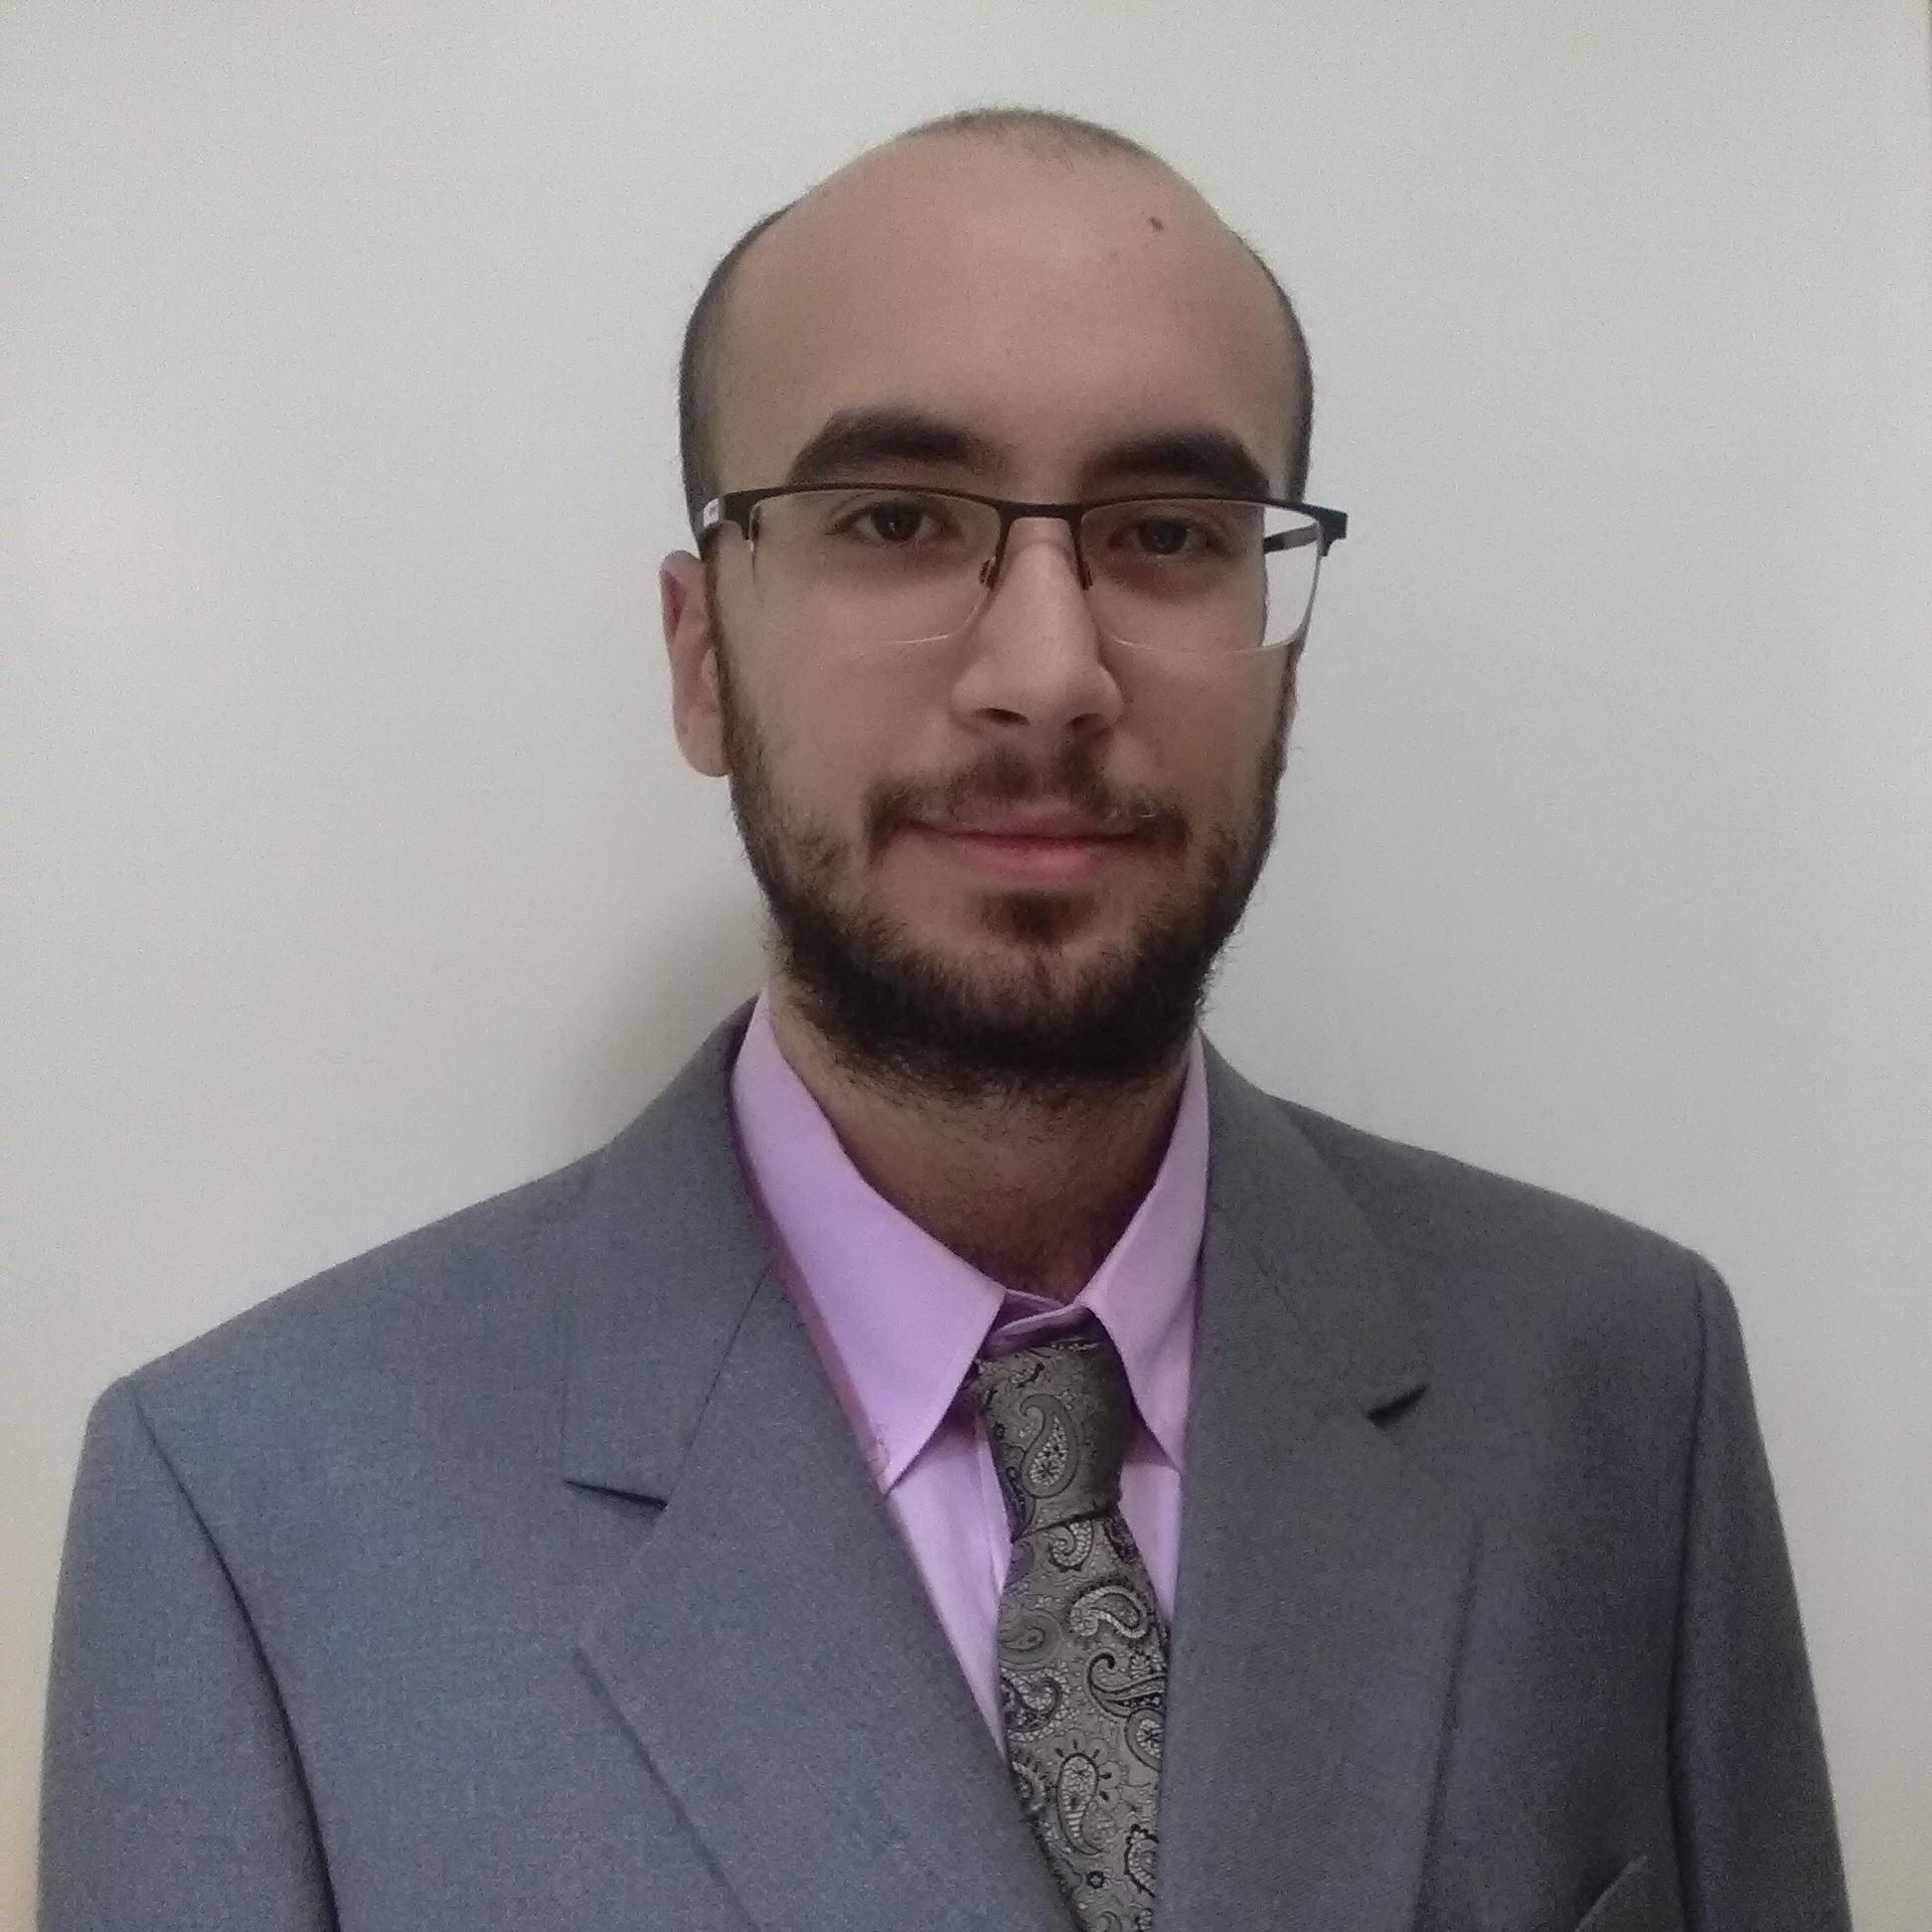
\includegraphics[width=5cm]{IMG_20190204_195706_ex.jpg}%
\columnbreak

\begin{flushright}
\textlatin{Name}: \textlatin{Iosif}

\textlatin{Surname}: \textlatin{Angelidis}

\textlatin{Birth}: \textlatin{June 16, 1993}

\textlatin{Address}: \textlatin{University of Athens, 157 84, Ilissia, Athens, Greece}

\textlatin{Mobile}: \textlatin{\href{tel:306947747843}{+30 694 7747 843}}

\textlatin{Phone}: \textlatin{\href{tel:302108843227}{+30 210 884 3227}}

\textlatin{e-mail}: \textlatin{\href{mailto:iosang@di.uoa.gr}{iosang@di.uoa.gr}}

\end{flushright}

\end{multicols}

\subsection*{Further Contact Means}
\addcontentsline{toc}{subsection}{Further Contact Means}

\begin{itemize}

\item \href{https://iosang.github.io}{Personal Website}

\item \href{https://www.facebook.com/metimdjai}{Facebook}

\item \href{https://www.linkedin.com/in/iosif-angelidis/}{LinkedIn}

\item \href{https://github.com/metimdjai}{GitHub}

\item \href{https://gitlab.com/metimdjai}{GitLab}

\item V-card: 
\includegraphics[scale=0.5]{qr.png}%

\end{itemize}

\newpage

\subsection*{Short summary}
\addcontentsline{toc}{subsection}{Short summary}

\begin{sloppypar}
	Iosif Angelidis was born in Cholargos, Attica, on 16/06/1993. He is a graduate of the Department
	of Informatics \& Telecommunications of the National and Kapodistrian University of Athens, his undergraduate 
	dissertation being in the area of ``Theoretical Informatics'', while he has completed his post-graduate studies in ``Information and Data
	Management''. He is a member of Management of Data and Information Knowledge Group
	(\href{http://www.madgik.di.uoa.gr}{MADgIK}) and the \href{http://ai.di.uoa.gr/}{AI group} of the University of Athens.
\end{sloppypar}

\begin{sloppypar}
	In the context of his MSc thesis, ``Named Entity Recognition and Linking in Greek Legislation'',
	under the supervision of professor Manolis Koubarakis and PhD Candidate Ilias Chalkidis, he
	developed and maintained a Named Entity Recognizer which recognizes and extracts persons,
	organizations, geo-political entities, legal references, public documents and unofficial
	geographical landmarks found in the Government Gazette by utilizing Neural Networks and Deep Learning
	technologies. These entities are being encoded as RDF data based on a Semantic Web ontology and
	then interlinked with other open public datasets (Greek Administrative Geography, Greek
	DBpedia Politicians, EUR-Lex) with Silk.
\end{sloppypar}

\begin{sloppypar}
	He has been a researcher, further developing, optimizing and maintaining the Named Entity Recognizer
	component he developed for the project \href{http://legislation.di.uoa.gr}{Nomothesi@} API, still contributing to the project when time allows. Also, he has worked as a researcher in Choronomothesia, 
	a parallel project with the goal of extracting geospatial information and coordinates from tables of legal documents of the National Printing Office of Greece.
\end{sloppypar}

\subsection*{Working experience}
\addcontentsline{toc}{subsection}{Working experience}

\begin{itemize}

\item Jul 1 2017 - Oct 7, 2019: Researcher:
	\begin{itemize}

	\item Developing, optimizing and maintaining the Named Entity Recognizer component of ``\href{http://legislation.di.uoa.gr}{Nomothesi@}''.

	\item Developer and researcher in ``Choronomothesia'', another project parallel to ``\href{http://legislation.di.uoa.gr}{Nomothesi@}'' with the goal 
	of extracting geospatial information and coordinates from tables of legal documents of the National Printing Office of Greece.

	\item Focus on various aspects of knowledge harvesting, representation, reasoning and analytics.

	\item Information extraction, web crawling, deep neural networks and machine learning, natural language processing.

	\item Member of Management of Data and Information Knowledge Group (\href{http://www.madgik.di.uoa.gr}{MADgIK}) and the \href{http://kr.di.uoa.gr/}{AI group} of the University of Athens.

	\end{itemize}

\item Jul 1, 2017 - Oct 31, 2017: Researcher/software developer in the project ``Copernicus App Lab'' (Horizon2020, EU Research and Innovation Programme).

\end{itemize}

\subsection*{Additional academic activities}
\addcontentsline{toc}{subsection}{Additional academic activities}

\begin{itemize}

\item Fall 2019: Teaching assistant in undergrad ``Artificial Intelligence'' course, National and Kapodistrian University of Athens, Department of Informatics and Telecommunications.

\item Fall 2018: Teaching assistant in undergrad ``Artificial Intelligence'' course, National and Kapodistrian University of Athens, Department of Informatics and Telecommunications.

\item Fall 2017: Teaching assistant in undergrad ``Artificial Intelligence'' course, National and Kapodistrian University of Athens, Department of Informatics and Telecommunications.

\item Fall 2016: Teaching assistant in undergrad ``Operating Systems'' course, National and Kapodistrian University of Athens, Department of Informatics and Telecommunications.

\item Fall 2015: Teaching assistant in Object Oriented Programming Lab for ``Object Oriented Programming'' undergrad course, National and Kapodistrian University of Athens, Department of Informatics and Telecommunications.

\item 2015: Supervision/development of educational material for ``Algorithms and Complexity'' and ``Operations Research'' undergrad courses, National and Kapodistrian University of Athens, Department of Informatics and Telecommunications.

\end{itemize}

\subsection*{Projects}
\addcontentsline{toc}{subsection}{Projects}

\begin{itemize}

\item Active developer of the platform \href{http://legislation.di.uoa.gr/}{Nomothesi@}, which functions as a portal of greek legislative text from all legal documents of the National Printing House. We extract legal and geospatial as well as textual references to entities, digitalizing this data as Semantic Web data by utilizing structured/semi-structured data with ontologies.

\item \begin{sloppypar}
\textbf{MSc Thesis} ``\href{https://pergamos.lib.uoa.gr/uoa/dl/frontend/en/browse/2766525}{Named Entity Recognition and Linking in Greek Legislation}''. Supervisors: Manolis Koubarakis (Professor, NKUA), Ilias Chalkidis (PhD Candidate, AUEB).
The main focus was on neural networks technologies in the area of natural language processing with the aim of extracting named entities (persons, organisations, legal references, geo-political entities, public documents and unofficial geographical landmarks), 
converting them into Semantic Web data and then linking them with other third party Semantic Web data (Greek Administrative Geography, Greek DBpedia ) using the tool Silk.

\end{sloppypar}

\item \begin{sloppypar}
\textbf{Undergrad Thesis} ``\href{http://efessos.lib.uoa.gr/applications/disserts.nsf/0f1ab5fee83fbb88c225770c0042ce4f/8da6d56136caaacec2257ea6004c9349?OpenDocument}{Capacitated Vehicle Routing with Time Windows}''. Supervisors: Alex Delis (Professor, NKUA), Panagiotis Liakos (PhD, NKUA). 
The main focus was addressing the titular problem, implement an adapted $A^{*}$ program to visualize the shortest paths between stops of the vehicles. To that end, geospatial information was being handled with a Postgres database with PostGIS functionality.

\end{sloppypar}

\item \begin{sloppypar}
``\href{https://bitbucket.org/Metimdjai/vrppd/src/master/}{Cooperative Routing and Scheduling of an Electric Vehicle Fleet Managing Dynamic Customer Requests}''. A work in collaboration with Alex Delis (Professor, NKUA) and Panagiotis Liakos (PhD, NKUA). 
The goal of this project was to develop an online algorithm that uses 3 distinct strategies to optimize routing and scheduling information of an electric vehicle fleet (which requests recharging) and compare all three. The problem addressed here is a new addition to the VRP-family of NP-hard problems.

\end{sloppypar}

\item Working on an \href{https://www.dropbox.com/sh/46dg71devshdvv1/AAAvynY_ZJJcsGwdC6ZGsQg5a?dl=0}{Android app} with RESTful services offering a similar functionality to Airbnb for ``e-Commerce'' class with geospatial functionalities, Google Maps and locating addresses.

\item Participation in a 3-member team where the representation of multiple social networks as graphs, graph quries (multi-threaded) and multiple metrics regarding communities and cliques finding were implemented (in C) for ``Software Development'' undergrad course.

\item Development of a \href{http://dl104.madgik.di.uoa.gr/eamgroup56/index.php}{lending library website} with user roles and shopping cart functionalities for ``Human-Computer Interaction'' undergrad course.

\item Geospatial data manipulation and production in the topics of LAI (Leaf Area Index) of Paris (from netCDF format), $NO_2$ , $O_3$ , $UV$ emissions in Europe and oil-spills in Sweeden for the \href{http://www.app-lab.eu/}{Copernicus App Lab} in addition to writing of scripts to automate tasks within the group and improve efficiency. 

\end{itemize}

\subsection*{Education}
\addcontentsline{toc}{subsection}{Education}

\begin{itemize}

\item 2016-2018: MSc degree in Information and Data Management, National and Kapodistrian University of Athens, Department of Informatics and Telecommunications. Grade: 9.39/10.0.

\item 2011-2016: Ptychion (4-year degree with thesis) in Computer Science - Theoretical Informatics, National and Kapodistrian University of Athens, Department of Informatics and Telecommunications. Grade: 9.34/10.0.

\item 2007: \textlatin{ECDL (Syllabus Version 4.0)} certificate in \textlatin{Databases, Concepts of IT, Word Processing, Presentations, Information and Communication, Spreadsheets, Using the Computer and Managing Files}.

\end{itemize}

\subsection*{Languages}
\addcontentsline{toc}{subsection}{Languages}

\begin{itemize}

\item English: \textlatin{Certificate of Proficiency in English, 2009 University of Michigan, First Certificate in English (Grade B), 2008 University of Cambridge.}

\item Greek: Native language.

\end{itemize}

\subsection*{Skills}
\addcontentsline{toc}{subsection}{Skills}

\begin{itemize}

\item Soft Skills: communication, team player, patient.

\item Programming Languages: \textlatin{C, C++, Java, Prolog, Haskell, Assembly (MIPS), Python, LUA, OpenGL, SPARQL/GeoSPARQL/stSPARQL, SMILE}.

\item Operating Systems: \textlatin{GNU/LINUX (Arch Linux, Manjaro, Debian, *buntu (Server), Fedora, OpenSuse, Kali/Backtrack, Arch, Mandriva, Mint, Debian, Slackware/Slackel, Puppy), Microsoft Windows (95, 98, 2000, XP, Vista, 7, 8, 10)}.

\item Shell Scripting: \textlatin{bash, fish, zsh, tcsh, csh}.

\item Applications Development \textlatin{RESTful Web Services, Android Studio development, TLS/SSL protocols, Bootstrap, Sweet Alert, Bootstrap Validator, bower, npm, HTML 5, CSS3, Ajax, jQuery, PHP, Javascript, Gradle, Maven, NodeJS, React, Redux}.

\item Server Management \& Databases: \textlatin{Apache Tomcat, Glassfish, Apache HTTP Server/XAMPP, PHPMyAdmin, MySQL Workbench, PostgreSQL/PostGIS, pgAdmin, Redis}.

\item Integrated Desktop Environments: \textlatin{Intellij, PyCharm, WebStorm, PHPStorm, Vistual Studio Code, Netbeans}.

\item Geospatial Systems: \textlatin{Sextant, Strabon}.

\item Version Control Systems: \textlatin{Mercurial, Git, CVS, GitHub, GitLab, Bitbucket}.

\item General: \textlatin{\LaTeX, Microsoft Office, Matlab, Gimp}.

\end{itemize}

\subsection*{Distinctions}
\addcontentsline{toc}{subsection}{Distinctions}

\begin{itemize}

\item 2011: Greek State Scholarships Foundation (IKY) scholarship for academic performance, 2011-2012.

\item 2002: second place certificate in backstroke 33m, Panellinios AC.

\end{itemize}

\subsection*{Publications}
\addcontentsline{toc}{subsection}{Publications}

\begin{itemize}

\item \textbf{\underline{I. Angelidis}, I. Chalkidis, C. Papaloukas and M. Koubarakis}. ``\textit{The Greek Legal Knowledge Graph: A Progress Report}''. Submitted, 2019. [\href{https://iosang.github.io/documents/Publications/2019/ISWC2019_Resources_126.pdf}{E-PRINT}].

\item \textbf{T. Beris, \underline{I. Angelidis}, I. Chalkidis, C. Nikolaou, C. Papaloukas, P. Soursos and M. Koubarakis}. ``\textit{Towards a Decentralised, Trusted, Intelligent and Linked Public Sector. A Report from the Greek Trenches}''. LDOW/LDDL workshop, The Web Conference (WWW 2019), San Francisco, CA, USA, 13 May, 2019. [\href{https://dl.acm.org/citation.cfm?doid=3308560.3317077}{PUB}][\href{https://iosang.github.io/documents/Publications/2019/www19companion-206.pdf}{E-PRINT}][\href{https://iosang.github.io/documents/Publications/2019/3317077.bib}{BIB}].

\item \textbf{\underline{I. Angelidis}, I. Chalkidis, C. Nikolaou, P. Soursos and M. Koubarakis}. ``\textit{Nomothesia: A Linked Data Platform for Greek Legislation}''. MIREL workshop, Luxembourg Logic for AI Summit (LuxLogAI 2018), Luxembourg, 17 September, 2018. [\href{https://ora.ox.ac.uk/objects/uuid:b19c1428-49db-402b-8afd-b8cf588e147d}{PUB}][\href{https://iosang.github.io/documents/Publications/2018/nomothesia-linked-data.pdf}{E-PRINT}][\href{https://ora.ox.ac.uk/objects/uuid:b19c1428-49db-402b-8afd-b8cf588e147d/export_record.bibtex}{BIB}].

\item \textbf{\underline{I. Angelidis}, I. Chalkidis and M. Koubarakis}. ``\textit{Named Entity Recognition, Linking and Generation for Greek Legislation}''. The 31st international conference on Legal Knowledge and Information Systems (JURIX 2018). Groningen, The Netherlands, 12-14 December‚ 2018. [\href{https://doi.org/10.3233/978-1-61499-935-5-1}{PUB}][\href{https://iosang.github.io/documents/Publications/2018/jurix2018.pdf}{E-PRINT}][\href{https://dblp.uni-trier.de/rec/bib1/conf/jurix/AngelidisCK18.bib}{BIB}].

\item \textbf{D. Punjani, K. Singh, A. Both, M. Koubarakis, \underline{I. Angelidis}, K. Bereta, T. Beris, D. Bilidas, T. Ioannidis, N. Karalis, C. Lange, D. Pantazi, C. Papaloukas and G. Stamoulis}. ``\textit{Template-Based Question Answering over Linked Geospatial Data}''. Geographic Information Retrieval (GIR 2018) workshop. Collocated with ACM SIGSPATIAL. Seattle, USA, 6 November, 2018.[\href{https://doi.org/10.1145/3281354.3281362}{PUB}][\href{https://iosang.github.io/documents/Publications/2018/template-based-GeoQA.pdf}{E-PRINT}][\href{https://dl.acm.org/downformats.cfm?id=3281362&parent_id=3281354&expformat=bibtex}{BIB}].

\item \textbf{P. Liakos, \underline{I. Angelidis} and A. Delis}. ``\textit{Cooperative Routing and Scheduling of an Electric Vehicle Fleet Managing Dynamic Customer Requests}''. Proceedings of the International Conference on Cooperative Information Systems (CoopIS), Rhodes, 28 October, 2016. [\href{https://link.springer.com/chapter/10.1007%2F978-3-319-48472-3_7}{PUB}][\href{https://iosang.github.io/documents/Publications/2016/LAD-Coopis16.pdf}{E-PRINT}][\href{https://dblp.uni-trier.de/rec/bib1/conf/otm/LiakosAD16.bib}{BIB}].

\end{itemize}

\subsection*{Research interests}
\addcontentsline{toc}{subsection}{Research interests}

\begin{itemize}

\item Deep Learning for NLP
\item Legal Text Analytics - Legislation Publishing, Contract Analysis
\item Information Extraction - Named Entity Recognition and Linking
\item Text Segmentation - Legal Text Segmentation, Zoning, Sentence Boundary Detection
\item Text Classification - Document/Sentence Classification
\item Self-supervised Document Classification
\item Data Augmentation
\item Legal Knowledge Representation - Legislation, Contracts
\item E-Government – Linked Open Data

\end{itemize}

\subsection*{Hobbies and interests}
\addcontentsline{toc}{subsection}{Hobbies and interests}

Apart from being a data scientist, I thoroughly enjoy travelling and visiting archaeological sites.

I strongly believe in the benefits of choosing swimming as a form of exercising over regular gymnastics. I used to go swimming for 6 years in boarding school and have taken a liking to it ever since. Of course, swimming does not have to be limited during summer, if one can endure the cold!

When forced indoors, I like talking about psychology, philosophy, mathematics, history and physics, or watching a good movie with friends (pretty much any genre, from horror to sci-fi to fantasy to comedy). Furthermore, I have been a gamer for a long time. I love playing almost all genres and fancy playing single player titles, or with friends. I definitely enjoy debating about games and their various aspects (gameplay, story, mechanics, gimmicksm etc.). Moreover, I am an aspiring DJ with a twist: I seek mostly music featured in games!

I like spending a good amount of my free time exploring the open source community, learning about new technologies and tweaking computer systems.

\end{document}
